\documentclass{article}
\usepackage[utf8]{inputenc}
\usepackage[english, ukrainian]{babel}
\usepackage{fontsize}
\usepackage{geometry}
\usepackage{amsthm}
\usepackage{amsfonts}
\usepackage{graphicx}
\usepackage[ruled]{algorithm2e}
\usepackage{hyperref}
\usepackage{biblatex}
\usepackage{csquotes}
\usepackage{mathtools}
\usepackage{amsmath}
\usepackage{amssymb}
\usepackage{bbm}
\usepackage{tabularx}
\usepackage{xcolor}

\usepackage{tikz}
\usetikzlibrary{decorations.pathmorphing}

\usepackage{enumitem}
\usepackage{nicefrac}

\usetikzlibrary{patterns}

\usepackage{diagbox}
\usepackage{longtable}

\usepackage{float}


\usepackage{enumitem}
\usepackage{nicefrac}

\usepackage{listings}
\definecolor{codegreen}{rgb}{0,0.6,0}
\definecolor{codegray}{rgb}{0.5,0.5,0.5}
\definecolor{codepurple}{rgb}{0.58,0,0.82}
\definecolor{backcolour}{rgb}{0.95,0.95,0.92}

\lstdefinestyle{mystyle}{
    backgroundcolor=\color{backcolour},   
    commentstyle=\color{codegreen},
    keywordstyle=\color{magenta},
    numberstyle=\tiny\color{codegray},
    stringstyle=\color{codepurple},
    basicstyle=\ttfamily\footnotesize,
    breakatwhitespace=false,         
    breaklines=true,                 
    captionpos=b,                    
    keepspaces=true,                 
    numbers=left,                    
    numbersep=5pt,                  
    showspaces=false,                
    showstringspaces=false,
    showtabs=false,                  
    tabsize=2
}

\lstset{style=mystyle}
\hypersetup{colorlinks=true, linkcolor=[RGB]{255, 3, 209}, citecolor={black}}

\graphicspath{ {../Images/} }

\begin{document}
    \begin{titlepage}
        \begin{center}
        $\newline$
        \vspace{3.3cm}
        
        {\LARGE\textbf{Лабораторна робота №5\\"Оптимізація нейронної мережі"}}
        \vspace{10cm}
        \begin{flushright}
            \textbf{Роботу виконав:}\\Климентьєв Максим \\3-го курсу\\групи ФІ-21
        \end{flushright}
        \end{center}
    \end{titlepage}
    \newpage

    \pagenumbering{gobble}
    \tableofcontents
    \cleardoublepage
    \pagenumbering{arabic}
    \setcounter{page}{3}

    \newpage

    \section{Опис параметрів оптимізації та мета оптимізації}
    \section{Опис експерименту, обраного алгоритму та отримані результати}
        \subsection{Обраний алгоритм}
            \begin{lstlisting}[language=Python, caption=DE]
def DE(pop_size, iterations, function, limits, ints):
    dim = len(limits)
    limits = np.array(limits)
    x_low = limits[:, 0]
    x_high = limits[:, 1]

    population = np.random.uniform(x_low, x_high, (pop_size, dim))

    if ints:
        for it in ints:
            population[:, it] = np.round(population[:, it])

    max_f = -float('inf')
    best_f = float('inf')
    best_pop = np.zeros(dim)

    # function calls = pop_size + iterations * pop_size
    fitness = np.array([function(X) for X in population])
    for iteration in tqdm(
        range(iterations),
        desc="Processing",
        unit="step",
        bar_format="{l_bar}{bar:40}{r_bar}",
        colour='cyan',
        total=iterations
    ):
        for i in range(pop_size):
            F = np.random.uniform(1e-6, 2)
            P = np.random.uniform(1e-6, 1)
            r = np.random.uniform(1e-6, 1, dim)
            x1, x2, x3 = np.random.choice(population.shape[0], size=3, replace=False)
            while np.all(population[x1] == population[i]) or np.all(population[x2] == population[i]) or np.all(population[x3] == population[i]):
                x1, x2, x3 = np.random.choice(population.shape[0], size=3, replace=False)
            mutant_vector = population[x1] + F * (population[x2] - population[x3])
            mutant_vector[r < P] = population[i][r < P]
            if ints:
                for it in ints:
                    mutant_vector[it] = np.round(mutant_vector[it])
            mutant_vector = np.clip(mutant_vector, x_low, x_high)
            mutant_fitness = function(mutant_vector)
            if fitness[i] > mutant_fitness:
                fitness[i] = mutant_fitness
                population[i] = mutant_vector.copy()
        el_min = np.argmin(fitness)
        if best_f > fitness[el_min]:
            best_f = fitness[el_min]
            best_pop = population[el_min].copy()
        el_max = np.max(fitness)
        if max_f < el_max:
            max_f = el_max

    return best_f, best_pop
            \end{lstlisting}

        \subsection{Фітнес функція}
            \begin{lstlisting}[language=Python, caption=Fitness Func]
def func(X):
    X = X.astype(int)
    amount_of_layer_1 = X[0]
    amount_of_layer_2 = X[1]
    amount_of_layer_3 = X[2]
    amount_of_one_dence = X[3]
    amount_of_one_filters = X[4]

    model_layers = [
        layers.Input(shape=(32, 32, 3)),
        data_augmentation
    ]

    for _ in range(amount_of_layer_1):
        model_layers.append(layers.Conv2D(int(amount_of_one_filters), (3, 3), activation='relu', padding='same'))
        model_layers.append(layers.BatchNormalization())
    model_layers.append(layers.MaxPooling2D(2, 2))

    for _ in range(amount_of_layer_2):
        model_layers.append(layers.Conv2D(int(amount_of_one_filters * 2), (3, 3), activation='relu', padding='same'))
        model_layers.append(layers.BatchNormalization())
    model_layers.append(layers.MaxPooling2D(2, 2))
    model_layers.append(layers.Dropout(0.3))

    for _ in range(amount_of_layer_3):
        model_layers.append(layers.Conv2D(int(amount_of_one_filters * 4), (3, 3), activation='relu', padding='same'))
        model_layers.append(layers.BatchNormalization())
    model_layers.append(layers.MaxPooling2D(4, 4))
    model_layers.append(layers.Dropout(0.4))

    model_layers.append(layers.Flatten())
    for _ in range(amount_of_one_dence):
        model_layers.append(layers.Dense(int(amount_of_one_filters * 8), activation='relu'))
    model_layers.append(layers.Dropout(0.5))
    model_layers.append(layers.Dense(10, activation='softmax'))

    model = tf.keras.models.Sequential(model_layers)
    summary_conv_and_last_dense(model)
    model.compile(optimizer=tf.keras.optimizers.Adam(learning_rate=0.001),
                loss=tf.keras.losses.CategoricalCrossentropy(),
                metrics=['accuracy', tf.keras.metrics.TopKCategoricalAccuracy(k=2, name="Top2")])
    history = model.fit(train, batch_size=batch_size, epochs=100, validation_data=(val), callbacks=callbacks)
    index = np.argmax(history.history['val_loss'])
    evaluation = model.evaluate(test)
    loss, acc, top2  = evaluation
    return (1.0 - acc) + loss

func_limits = [[1, 4], [0, 4], [0, 4], [1, 4], [16, 64]]
            \end{lstlisting}

        \subsection{Порівняння результатів (до оптимізації параметрів нейронних мереж та після)}
            \begin{tabular}{ |c|c|c|c| }
                \hline
                Тип & Час & Точність & Втрати\\ 
                \hline
                До & 30 & 70 & 90\\
                \hline
                Після & 34 & 80 & 58\\
                \hline
            \end{tabular}
    \newpage
            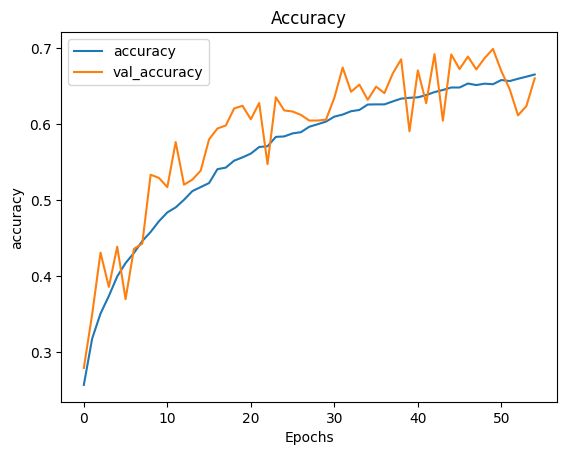
\includegraphics[scale=0.5]{before_acc.png}
            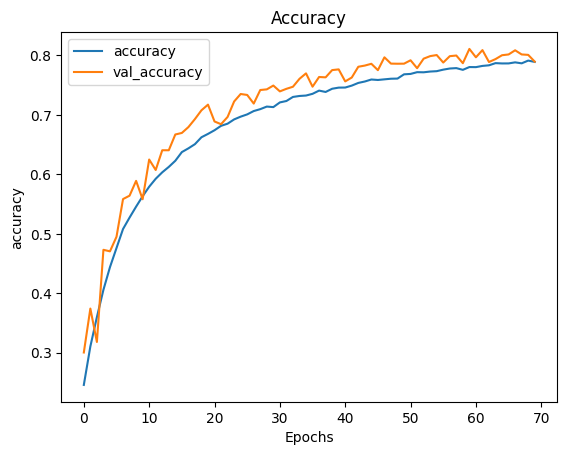
\includegraphics[scale=0.5]{after_acc.png}
    \newline
            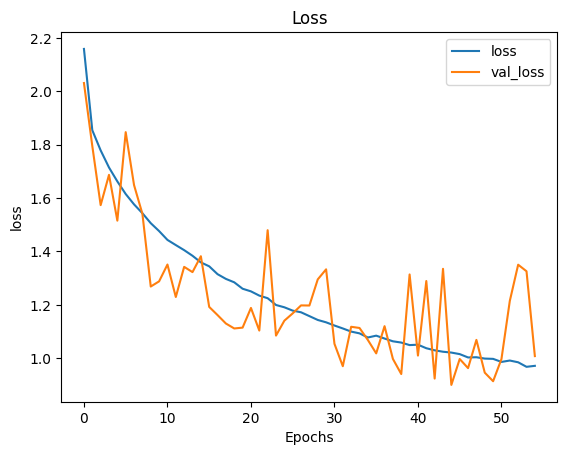
\includegraphics[scale=0.5]{before_loss.png}
            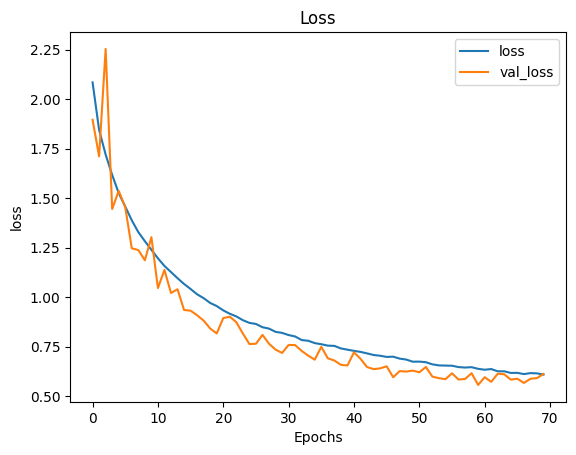
\includegraphics[scale=0.5]{after_loss.png}
    \newpage

        \subsection{Час виконання (пошук оптимального рішення та інше)}
            \begin{tabular}{ |c|c| }
                \hline
                Тип & Час (хв)\\ 
                \hline
                Пошук оптимального рішення & 1500-2000\\
                \hline
                Побудова ландшафту & 2000-4000\\
                \hline
                Інше & 30\\
                \hline
            \end{tabular}
    \section{Висновки}
            Модель стає кращою як по збільшенню точності, так і по зменшенням втрат
            Також чим менше дропаут, та чим більше фільтрів тим точніше
    \newpage
            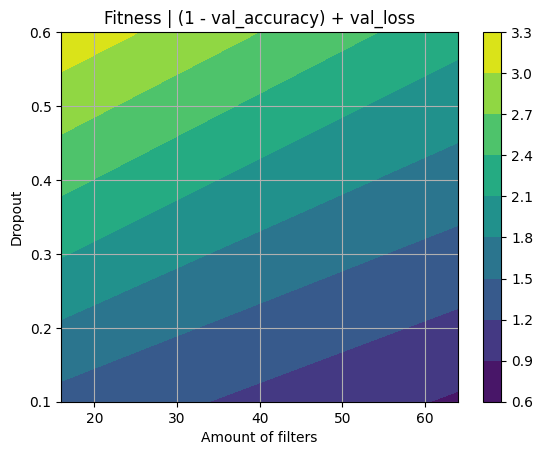
\includegraphics{Landscape.png}
\end{document}